\subsection{C-Library cddlib pour l'énumération des Sommets}
\subsubsection{Définition}

La bibliothèque cddlib est une implémentation C de la méthode double description de Motzkin et al.Pour générer tous les sommets(c’est-à-dire les points extrêmes) et les rayons extrêmes d’un polyèdre convexe général dans $ \reels^{d}$ donnée par un système d’inégalités linéaires:  

\begin{equation}
     P= \{ x=({x}_{1}, \ldots, {x}_{d})^{T}  \;: \;Ax \leq b  \}     
\end{equation}

% * <assale.adje@gmail.com> 2018-07-27T11:59:59.141Z:
% 
% Attention la relation d'ordre n'est pas la même il ne faut plus utiliser le même signe d'inégalité
% 
% ^.
où $A$ est une matrice réelle $m$ x $d$ donnée, $b$ est un m-vecteur donné et 0 est le m-vecteur de tous les zéros.


\subsection{ H-representation \& V-polyhedron}

Un polyèdre peut être décrit par une liste d'inégalités (H-representation) ou par une liste de ses sommets + rayons extrêmes (V-representation ) où "+" est la somme de \textit{Minkowski}\footnote{(en géométrie) une opération sur les parties d'un espace vectoriel. À deux parties $A$ et $B$ elle associe leur ensemble somme, formé des sommes d'un élément de $A$ et d'un élément de $B$}. Cddlib\cite{cdd/cddplus} permet de convertir un programme qui représente un polyèdre par H-representation en son V-representation, et vice versa.Ces problèmes sont connus respectivement au niveau de l’énumération des sommets et des problèmes de \href{http://le-terrier-de-lapineige.over-blog.com/2014/09/bm-c-comme-convex-hull-un-outil-de-modelisation-polyvalent.html}{coque convexe}.
\newpage
\subsection{ formats de fichiers avec l'implémentation sur un exemple}
% * <assale.adje@gmail.com> 2018-07-27T12:02:53.141Z:
% 
% Copier-coller!!
% 
% ^.
L’entrée pour Cddlib est une H-représentation ou V-representation d’un polytope.Ces fichiers ont les formats suivants:
 \begin{figure}[ht]
	\centering
	\begin{subfigure}{.20\textwidth}
		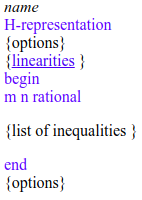
\includegraphics[width=\textwidth,scale=0.7]{images/H_representation.png}
		\caption{H-Représentation}
		\label{fig:h_represt}
	\end{subfigure}\hfill%
	\begin{subfigure}{.33\textwidth}
		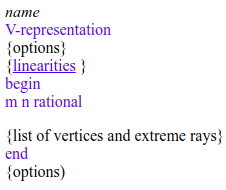
\includegraphics[width=\textwidth,scale=0.7]{images/V_representation.png}
		\caption{V-Représentation}
		\label{fig:v_represt}
	\end{subfigure}\hfill%
	\caption{H-Représentation \& V-Représentation}
	\end{figure}
    
    
    
    \subParagraphe{Représentation en demi-espace(H-representation) }
    
    \vspace*{.5cm}
    
La H-representation d'un polytope convexe $S$ n'est qu'un ensemble d'inégalités linéaires correspondant à l'intersection des demi-espaces: $$S = (x \; |\; Ax\leq b)$$
 Il est toujours possible de normaliser la représentation pour que les composantes de b soient 1 ou 0. Lorsque toutes ces composantes sont nulles, le polyèdre est un cône convexe polyédrique pointé à l'origine. Quand tous les composants de b sont des uns, rien ne peut être dit avec certitude Mais, à l'inverse, pour un polytope on a seulement un dans le vecteur colonne de son H-representation. Nous nous retrouvons donc avec le vocabulaire suivant:
 
 $$Polyedre: P=\{(x \; | \; Ax\leq b)\} $$
 $$Cone \; polyedrique: P=\{(x \; | \; Ax\leq 0)\}$$
$$Polytope: P=\{(x \; | \; Ax\leq 1)\}\\ $$

Prenons en exemple ces inégalités:
 \begin{equation}
      1+{x}_{1} \succeq 0 \;\;\; \;\;\;  1+{x}_{2}\succeq 0  \;\;\;\; \; \; 1-{x}_{1} \succeq 0 \;\; \;\; \;\;   1-{x}_{2} \succeq 0 
\end{equation}

ces inégalités sont entrées comme la ligne 
\begin{equation}
      {a}_{0} \; {a}_{1}, \ldots ,{a}_{n-1}    
\end{equation}

et qui serait représenté par le fichier d’entrée 


 \begin{figure}[ht]
	\centering
\fbox{	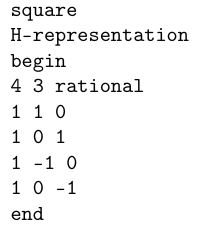
\includegraphics[width=.2\textwidth]{images/exempl-Hrepst.png}}
	\label{fig:ex_hreprest}
\end{figure}

\subParagraphe{Fichier V-representation}

\vspace*{.5cm}

La représentation de sommet (V-representation) d'un polyèdre le décrit en termes de points (sommets), comme il génère des vecteurs appelés rayons. Informellement, les sommets sont les limites "finies" du polyèdre, tandis que les rayons sont les "infinis". Un polytope n'a que des sommets, tandis qu'un cône polyédrique ne contient que des rayons. Formellement, les points x du polyèdre sont décrits par:
$$x=conv(V)+coni(R)$$

où $conv$ désigne la coque convexe d'un ensemble de sommets $V=\{ v_1,\ldots, v_p \}$

tandis que $coni$ est la coque conique d'un ensemble de rayons $R=\{ r_1,\ldots, v_q \}$


chaque sommet (voir Figure \ref{fig:v_represt}) est donnée sous la forme:
\begin{equation}
      1 \;{v}_{0} \; {v}_{1}, \ldots ,{v}_{n-1}    
\end{equation}

chaque rayon est donnée sous la forme 

\begin{equation}
      0 \;{r}_{0} \; {r}_{1}, \ldots ,{r}_{n-1}    
\end{equation}

où  $ 0 \;{r}_{0} \; {r}_{1}, \ldots ,{r}_{n-1}$ est un point sur le rayon.


Il doit y avoir au moins un sommet dans chaque fichier. Pour les polyèdres bornés, il n’y aura pas de rayons entrés.\\

Par exemple, l’entrée de fichier V-representation serait représenter comme suit: 

\begin{figure}[ht]
	\centering
\fbox{	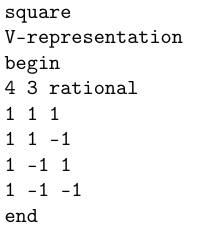
\includegraphics[width=.2\textwidth]{images/exem-Vreprst.png}}
	\label{fig:ex_Vreprest}
\end{figure}

où (1,1), (1,-1), (-1,1), (-1,-1) représentent les sommets.\\


La conversion d'un sommet à une représentation demi-espace(H-representation) est connue sous le nom de problème d'énumération de facette, tandis qu'à l'inverse, la conversion d'un demi-espace en représentation de sommet(V-representation) est le problème d'énumération de sommet. Ces deux problèmes sont en réalité équivalents lorsqu'ils sont soumis à une formulation mathématique appropriée et peuvent être résolus en utilisant la méthode de la double description. La bibliothèque \textit{cdd }fournit une implémentation C de cet algorithme.

\subsection{Opérations matricielles en C}

 Ceci est notre ensemble de bibliothèques C pour faire des opérations matricielles simples et l'algèbre linéaire (résolution de systèmes d'équations linéaires, de valeurs propres et de matrices inverses ainsi le calcule de la norme maximale d'une matrice de données).\\
 
 Voici les opérations de base que cette bibliothèque espère accomplir:
 
 \newpage
 \vskip .6cm
 \begin{itemize}
     \itemperso{Fichier Matriciel IO}
      \begin{itemize}
          \subitemperso{Matrix Read} pour lire une matrice à partir d'un fichier.
          \subitemperso{Matrix Copy }pour dupliquer une matrice existante.
          \subitemperso{Matrix Make} pour créer une matrice n-by-p de Zeros.
          \subitemperso{Matrix Free}pour libérer de la mémoire.
          \subitemperso{Matrix Write}pour écrire dans un fichier.
          \subitemperso{Matrix Print} pour afficher une matrice sur l'écran.
         
      \end{itemize}
     \itemperso{Opérations matricielles simples}
     \begin{itemize}
        
  \subitemperso{Identity Matrices}.
  \subitemperso{Matrix power} $A^{B}$ calcule $A$ en puissance $B$ et renvoie le résultat en $C$.
  \subitemperso{Matrix Trace} Somme des éléments le long de la diagonale.
  \subitemperso{Matrix Transpose} Pour retourner une matrice le long de la diagonale.
  \subitemperso{Matrix Mean} renvoie la moyenne de chaque colonne dans une matrice.
  \subitemperso{Matrix Multiplication}.
  \subitemperso{Matrix Scaling}.
  \subitemperso{Matrix Covariance}.
  \subitemperso{Matrix Dot Product}.
  \subitemperso{Matrix Dot Diagonal} calcule le produit scalaire des diagonales de deux matrices.
  \subitemperso{Singular Value Decomposition}.
  \subitemperso{Gram-Schmidt} Pour l’orthonormalisation d’un ensemble de vecteurs.
  \subitemperso{The Power Method} Pour déterminer la plus grande valeur propre d'une grande matrice.
  \subitemperso{Francis QR Step}.
  \subitemperso{Eigenvalues}. 
  \subitemperso{L2-norm distance measures} similaire au pdist de Matlab.
  \subitemperso{ LU Decomposition of a matrix}.
  \subitemperso{Matrix Determinates}.
  \subitemperso{Matrix Inverts}.
  \subitemperso{Matrix Solver} Résout un système d'équations linéaires en utilisant la décomposition LU. Cela nécessite une matrice $A:n \times n$ et une matrice $B:n \times p$, où $A * X = b$ L'algorithme renvoie $X$, qui sera une matrice $n \times p$. Cet algorithme est décrit à la page 121 du livre \textit{Matrix Computations} \cite{H.Golub} Golub and Loan).
  \subitemperso{Matrix Inverse}. 
  \subitemperso{Matrix Max\_Norm} Cette fonction trouve la norme maximale d'une matrice, Cette norme est simplement le plus grand élément absolu de la matrice.
     \end{itemize}
 \end{itemize}
 
 \begin{itemize}
     \itemperso{Toujours agréable d'avoir}
     \begin{itemize}
         \subitemperso{Quicksort.}
     \end{itemize}
     
 \end{itemize}



 \subsection{Calcul de valeurs propres et de vecteurs propres}
 
  \subsubsection{Présentation}


Les valeurs propres (EigenValues) d'une matrice $A$ carré $n$x$n$ sont le nombre $n$ réel ou complexe $\lambda_{i}$ tel que l'équation $Ax =\lambda x$ a des solutions non triviales ${\lambda}_{1},{\lambda}_{2},{\lambda}_{3},\ldots, {\lambda}_{n}$.\\
Si $A$ est symétrique, alors les valeurs propres sont réelles.\\
En réécrivant $Ax = \lambda x$ comme $(A - \lambda I) x = 0$, les $\lambda$ sont les racines de l'équation du déterminant polynomial $(A - \lambda I) = 0$.\par

Les vecteurs propres (EigenVectors) de $A$ sont l'ensemble des N-vecteurs $x = u_{i}$ (certains livres utilisent $q_{i}$) qui sont les solutions non triviales de $Ax = {\lambda}_{i}x$.C'est-à-dire $Au_{i} = {\lambda}_{i}u_{i}$ pour chaque $i$.\\
Rappelons que, si aucun des ${\lambda}_{i}$ n'est répété, les vecteurs propres normalisés $( \| u \|_{2} =1)$ forment un ensemble orthonormé. c'est-à-dire $ {u_{i}}^{T} u_{i}= 1$, mais $ {u_{i}}^{T} u_{j}= 0$ pour tout $i \neq j$.\\
Tout vecteur $x$ peut être exprimé en fonction de cet ensemble orthonormé:
$$x=a_{1}u_{1}+a_{2}u_{2}+ \ldots + a_{n}u_{n}.$$

Pour la recherche des valeurs propres d'une matrice carrée, chacun à sa petite méthode et le but est d'aller le plus vite possible sans se tromper.Dans cette partie, on va faire un petit tour d'horizon des deux méthodes utilisées.

\subsubsection{EigenValue en deux méthodes différentes}

\subParagraphe{Méthode de la puissance itérée (PowerMethod)}

\vspace*{.5cm}

 La méthode Power est la méthode classique pour calculer les plus grandes valeurs propres d'une matrice. La méthode est motivée par la propriété que si on multiplie un vecteur par une matrice, la contribution du vecteur propre correspondant à la plus grande valeur propre (en valeur absolue) a augmenté plus que la contribution des autres vecteurs propres. Si le vecteur est multiplié un grand nombre de fois par la matrice, la contribution de ce vecteur propre dominera, de sorte que le vecteur d'itération qui en résulte se rapprochera de ce vecteur propre( Ceci nous a été décrit dans un cours Randomized Algorithms\cite{M.goodrich}). Nous arrivons donc à l'algorithme suivant:
 
 
  \begin{itemize}
 \itemperso{1.} Début.
 \itemperso{2.} Définir la matrice $X$.
 \itemperso{3.} Calculer $Y = AX$.
 \itemperso{4.} Trouvez l'élément le plus grand dans l'amplitude de la matrice $Y$ et attribuez-le à $K$.
 \itemperso{5.} Calculez la nouvelle valeur $X = (1 / K) * Y$.
 \itemperso{6.} Si $[K_{n} - K_{n-1}]> \delta$, passez à l 'étape 3.
 \itemperso{7.} Arrêtez.
 \end{itemize}
 
 \subParagraphe{FrancisQRstep}
 
 \vspace*{.5cm}
 
 Cet algorithme effectue l’étape Francis QR Step pour trouver les valeurs propres(et éventuellement les vecteurs propres) d’une matrice carrée.
Le traitement de l'algorithme QR dans  \href{http://people.inf.ethz.ch/arbenz/ewp/Lnotes/2010/chapter3.pdf}{ces notes de cours} sur le calcul de la valeur propre à grande échelle est justifié à deux égards. Tout d'abord, il y a bien sûr des problèmes de valeurs propres importantes, voire énormes. Deuxièmement, l'algorithme QR est utilisé dans la plupart des autres algorithmes pour résoudre les petits problèmes de valeurs propres auxiliaires voire «internes».Actuellement, on a cette méthode pour tester l’approche. 

\subsubsection{Entrées du programme}

  \begin{lstlisting}[language=C++]
#include <stdio.h>
#include "matrix.h"
#include "eigen.h"

int main(int argc, char** argv) {

    matrix* a = readMatrix(argv[1]);//a=[0.75 1;0.36 0.5]
    matrix* evec;
    double eigenvalue; 
   
 /*===================================================================
 * francisQRstep
 * This algorithm performs the Francis QR Step to find the eigen values of a square matrix.
 * We just read this technique in the article "The QR Algorithm". Currently we have this method to test the approach.
 =====================================================================*/
    
    matrix* e = francisQRstep(a);
    printMatrix(e);
    eigenvalue = e->data[ e->height - 1 ];
    printf("Largest eigenvalue: %f (francis qr step)\n", eigenvalue);

/*==================================================================
 * powerMethod
 *This algorithm determines the largest eigenvalue of a matrix using the power method
 *This was described in a Randomized Algoirthms course.
 *===================================================================*/

    eigenvalue = powerMethod_largest(a);
    printf("Largest eigenvalue: %f (power method) \n", eigenvalue);
    
/*==================================================================
 * eigenvector
 * This algorithm determines the eigenvector of a matrix given an eigenvalue.
 *=================================================================*/
 
    evec = eigenvector(a, eigenvalue);
    printMatrix(evec);
    
       //clean up
    freeMatrix(evec);
    freeMatrix(e);
    freeMatrix(a);
    return 0;
} \end{lstlisting}



 \subsubsection{Sortie du programme}  
 
 \begin{figure}[ht]
	\centering
\fbox{	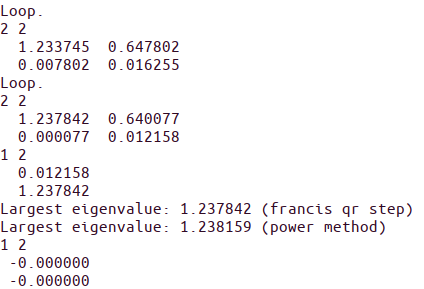
\includegraphics[width=.4\textwidth]{images/eigen-value.png}}
	\label{fig:ex_Vreprest}
	\caption{La plus grande valeur propre retournée(francisQRstep \textit{VS} powerMethod)}
\end{figure}





